\documentclass[12pt,a4,xcolor=table]{article}
\usepackage[margin=1in]{geometry}
\usepackage{hyperref}
\usepackage{multicol}
\usepackage{multirow}
\usepackage[usenames,dvipsnames,svgnames,table,xcdraw]{xcolor}
\usepackage[rightcaption]{sidecap}
\usepackage{enumitem}
\usepackage{tikz}
\usetikzlibrary{trees}
\usepackage{array,booktabs}
\usepackage{pgfgantt}
\usepackage{rotating}
\usepackage{amssymb}
\usepackage{fdsymbol}
\usepackage{listings}
\usepackage{color}
\usepackage[dvipsnames]{xcolor}
\usepackage{wrapfig}
\usepackage{makecell}
\usepackage[normalem]{ulem}
\graphicspath{ {./figures/} }
\useunder{\uline}{\ul}{}
\usepackage{etoolbox}
\patchcmd{\thebibliography}{\section*{\refname}}{}{}{}
\title{Literature Review}
\author{}
\date{}

\begin{document}
	\begin{titlepage}
		\newcommand{\HRule}{\rule{\linewidth}{0.5mm}}
		\center
		\Large Electronics and Computer Science\\
		\Large Faculty of Physical Sciences and Engineering\\
		\Large University of Southampton\\[1.5cm]
		\Huge Anna Kutseva\\
		{\large 11 December,2018}\\[3cm]
		\HRule \\[0.4cm]
		\textsc{{\huge Exploring Turing Machine Simulations on Social Machines }}\\[0.3cm]
		\HRule \\[1.5cm]
		\LARGE Project supervisor: Thanassis Tiropanis \\
		\LARGE Second examiner: Adam Prugel-Bennett \\[1.5cm]
		\Large A project progress report submitted for the award of BSc Computer Science \\[1.5cm]
	\end{titlepage}
	\tableofcontents
	\thispagestyle{empty}
	\newpage
	\begin{abstract}
		The more popular and widely used certain web applications and services are, the more their content, functionality, and performance revolve around their users' actions.
		The concept of social machines is becoming more and more relevant with the vast expansion of the World Wide Web, as well as the increasing user involvement in its augmentation. The basis of the former, as first suggested by Tim Berners Lee, is weaving together the creative input of various individuals with the technical processing of machines.
		However, at the time of writing there is no known way to simulate these interactions which fundamentally underpin our usage of the internet as a source of information. Addressing this issue, the project is going to identify the core theoretical components of social machines and build a tool for simulating the dialogue between man and machine based on formally defined behaviours.
		This will be done by implementing one possible architecture and evaluating its applicability in mimicking real-life situations.
		Being able to observe socio-computational scenarios a system goes through could serve a deeper insight into the possible consequences of past, or hypothetical, design choices.
	\textcolor{red}{
		\\- Mention Turing!
		\\- outro sentence!	
	}
	\end{abstract}
	\thispagestyle{empty}
	\clearpage
	%\section*{Acknowledgements}
	%\thispagestyle{empty}
	%\clearpage
	\pagenumbering{arabic} 
	
	\section{Introduction}
	\subsection{Problem}
	\textcolor{red}{
		Large and complex online systems no longer only involve servers performing deterministic operations; there are cases where human input is an integral part in the completion of a certain task or advancing through a continuous process. With the rise of the World Wide Web people have been prompted to not only interact with each other online, but with systems they can contribute to. Such systems can be classified as social machines, as the dependency of their states on the non-deterministic nature of human participants conveys the interweaving of computer logic with real-life knowledge.
		Social machines have received a fair amount of academic attention in the form of designs and frameworks to help form a more rigorous outline of their structure and behaviour. However, there are fewer attempts in developing related software for further experimental exploration, and no known simulator of a formally defined social machine scheme exists at the time of writing this report.
	}
	\subsection{Goals}
	\textcolor{red}{
		This project aims at finding a way to simulate such environments, thus evaluating the feasibility of modelling social machine components using Turing machine simulations.
		There are three major stages this objective has:
		\begin{enumerate}[label=\textit{Stage \arabic*}]
			\item Gather a selection of models and classification frameworks to formally define the different behaviours of each component implementation
			\item Find an appropriate open source Turing Machine simulation framework and extend it with implementations of these extra models
			\item Assess the performance and accuracy of these simulations based on theoretical input scenario data or example data if such is available.
		\end{enumerate}
		Though largely sequential as each stage depends on the previous, it is acknowledged that there will be some amount of overlap as concepts require clarification or alignment moving forward.
	}

	\subsection{Scope}
	\textcolor{red}{
		Following the literature review it would seem that most previous endeavours into the domain have remained purely theoretical and as such evaluation metrics will be relatively basic. The lack of practical experiments to lean on means that this project will focus primarily on the implementation rather than attempting to populate an expansive data set for testing all possible metrics and scenarios moving forward. To further limit the goal into a feasible experiment to run within the time frame, existing software for simulating Turing machines will be built upon, thus ensuring all the effort is concentrated on implementing original features, rather than developing a full simulator from scratch.
	}

	\textcolor{red}{
		\subsection{Structure of report}
	}
	\textcolor{red}{
		\subsection{Statement of Ethics}
		\begin{itemize}
			\item No need for statistical data gathering
			\item No need for human participation
		\end{itemize}
	}

	
	\section{Related Work}
	\paragraph{Motivations}
	\textcolor{red}{
		Why do you think Oracle machines are useful? \\
		Why is it bad that we can't simulate them? \\
		How will it help if you are able to simulate them?
	}
	\subsection{Literature Review}
	\subsubsection{Turing Machines}
	\textcolor{red}{
	\paragraph{Concept}
	The initial concept of the now famous Turing machine was created as a mechanism to prove that the Entscheidungsproblem is unsolvable \cite{Turing1936} but turned out to have many further applications. While Alan Turing's take of machine learning \cite{Turing1969} %original was from 1948 
	and human-like conciousness \cite{Turing1950}, although possible to emulate with state machines, were way ahead of their time, his model of abstract a(utomatic)-machines contributed greatly on the foundations of the computer science field.
	\paragraph{Formal definition}\hfill\\
	$M=\langle Q,\Gamma ,\Sigma,b,q_{0} ,\delta ,F\rangle$
	\cite{Hopcroft1979} where:
	\begin{multicols}{2}
		\begin{itemize}
			\item Q - the finite set of states
			\item $\Gamma$ - the complete alphabet set
			\item $\Sigma \subseteq \Gamma \setminus \{b\}$ - the set of tape symbols
			\item $b\in\Gamma$ - the blank symbol
			\item $q_{0}\in Q$ - the start state
			\item $\delta :(Q\setminus F)\times \Gamma \rightarrow Q\times \Gamma -  \times \{L,R\}$ - the transition function
			\item $F\subseteq Q$ - the set of accepting states\footnote{There exist variations of the definitions with regards to accepting and rejecting states, but they are all proven to be equivalent. This one follows the definition taken from 'Introduction to automata theory, languages, and computation'\cite{Hopcroft1979}. In section \ref{sec:omega} single \textit{accept} and \textit{reject} states are used instead, following the 'Introducing the $\Omega$-machine' paper\cite{Zhang2014}}
		\end{itemize}
	\end{multicols}
	}
	\subsubsection{O-machines}
	\textcolor{red}{
	There exists a less known idea for an abstract machine by Turing, which was introduced in his PhD thesis - the \textit{o-machine}. Similarly to a-machines\footnote{The Turing machines that are familiar to the greatest number of people in the field.}, o-machines can be described through tables. The main difference between o-machines and other abstract machines, such as a-machines, is the black box element, called an 'oracle'. The latter's definition in is not expanded on in Turing's paper, beyond being depicted as \textit{"some unspecified means of solving number theoretic problems"}\cite{Turing1938}. No details on the internal configuration of an instance of such a machine are available. The o-machine is equipped with one or more oracles, each of which can perform a primitive operation that returns the values of a non-Turing-machine-computable\footnote{In other words - number theoretic} function\cite{Copeland1998} in the form \[ p:\mathbb{N}\mapsto \mathbf{2} \]
	\begin{wrapfigure}{r}{0.2\textwidth}
		\centering
		\raisebox{0pt}[\dimexpr\height-0.9\baselineskip\relax]{\includegraphics[width=0.2\textwidth]{cropart}}%
		\caption[short text]{text}
	\end{wrapfigure}
	The black box nature of the oracles allows for assumptions about what o-machines could represent. One proposed interpretation is that a human brain can be simulated by an o-machine\cite{Copeland1998}. Within the context of modelling social machines, a set of oracles can be utilised as stand-ins for a group of human individuals. Any taken series of actions in a certain environment can be broken down to a set of decision problems, which will then be emulated by the two-valued functions of the oracles.
	\clearpage
	\begin{multicols}{2}
		[According to van Melkebeek\cite{Melkebeek}, an o-machine has the following components:]
		\begin{itemize}
			\item Shared with traditional TMs:
			\begin{description}
				\item[work alphabet] a set of symbols which can be written on the work tape
				\item[work tape] an infinite sequence of cells that can either be empty or contain a symbol from the tape alphabet
				\item[read/write head] a component located on a single tape cell at a time that can move left or right on the work tape, as well as read and write\footnote{or delete by placing a 'blank symbol'} symbols on it
				\item[control mechanism] responsible for performing actions such as moving the head, manipulating data and switching states\\\\\\
			\end{description}\columnbreak
			\item Additional components
			\begin{description}
				\item[oracle alphabet] a set of symbols that may or may not be different from the work alphabet
				\item[oracle tape] a semi-infinite tape of cells that can either be empty or contain a symbol from the oracle alphabet
				\item[oracle head] acts the same way as the RW head, but on the oracle tape
				\item[\texttt{ASK} and \texttt{RESPONSE} states] when the oracle enters \texttt{ASK} state, the current oracle tape contents are taken as a problem instance and given as an input to the oracle, which, upon finding the problem solution, replaces the work tape contents with its output; the head is moved to the beginning of the tape; state is set to \texttt{RESPONSE}
			\end{description}
		\end{itemize}
	\end{multicols}
	\paragraph{Summary}
	}	
	\subsubsection{Interaction}
	\textcolor{red}{
	Machines established solely on the basis of computable functions fall flat in modelling present-day computing, considering its trademarks are \textit{interaction} and \textit{reactivity}\cite{Goldin2004}. Having in mind the notion that interactive systems are more expressive than algorithmic ones\cite{Wegner1997}, we can look into evolving the traditional models into something more applicable to the current technological circumstances. \\\\
	The TM component of the project can be modelled like a Persistent Turing Machine, with a work and output tapes\footnote{Possibly an input tape as well, if determined as needed.}.
	}
	\subsubsection{Social Machines}
	
\textcolor{red}{
	The concept of a social machine revolves around the idea of collaborative problem solving \cite{Luczak-Rosch2015}. As defined by  Tim Berners-Lee, they are \textit{"processes in which the people do the creative work and the machine does the administration"}\cite{berners2001weaving}.\\\\The combination of predefined machine transitions and probabilistic human input allows for introducing a plethora of outcomes for even a single system if it gets exposed to different selections of people. This is closer to the reality of modern computing, than the strict schemas of Turing machines. \footnote{While non-deterministic counterparts of the latter exist, they are closer in potential to being abstract machines than actual representations of the ever-increasing and practically boundless total of branches each interaction presents in real time.}\\\\By reinforcing connection and collaboration between people, social machines indicate existing relationships among themselves. One type of association they exhibit is belonging to one another and thus having types that can be arranged in a hierarchical tree with the World Wide Web as an infrastructure being its root (See Figure \ref{fig:sm-tree}) \cite{Shadbolt2009}.	
	\begin{SCfigure}[1][h!]
		\centering
		\tikzstyle{every node}=[draw=black,thick,anchor=west]
		\tikzstyle{selected}=[draw=red,fill=red!30]
		\tikzstyle{optional}=[dashed,fill=gray!50]
		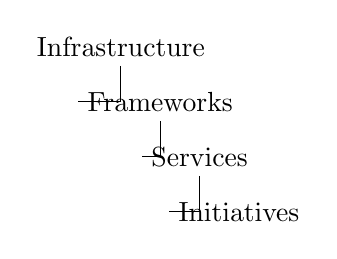
\begin{tikzpicture}[%
		grow via three points={one child at (0.5,-0.7) and
			two children at (0.5,-0.7) and (0.5,-1.4)},
		edge from parent path={(\tikzparentnode.south) |- (\tikzchildnode.west)}]
		\node {Infrastructure}
		child { node {Frameworks}
			child { node {Services}
				child { node {Initiatives}
				}
			}
		};
		\end{tikzpicture}
		\caption{Granularity levels of social machines - \textit{Initiatives} (a.k.a. \textit{Projects}) using \textit{Services} built upon \textit{Frameworks} contained into the Infrastructure}
		\label{fig:sm-tree}
	\end{SCfigure}
}
\textcolor{red}{
	\paragraph{The emerging web of social machines}
	Studies the relationships between SMs\cite{Silvio2010}
	\paragraph{From the semantic web to social machines: a research challenge for AI on the World Wide Web}
	Connects the semantic web with SMs and provides future goals\cite{Hendler2009}
}
\textcolor{red}{
	\subsubsection{Social Machine and Computation Examples}
	Given a lack of evaluation data found during the literature review, a few real-world social machines have been identified with the possibility of simulation by reducing the domain and action set of the oracles and machine respectively to a few representative outcomes (both positive and negative):
	\paragraph{Wikipedia}
	Serving as one of the most well-known cases of social machines, Wikipedia would not exist without the endless flow of human input. It confirms the capacity of social computation by being the largest encyclopedia in existence, that is being updated at such a rate that physically publishing its content is absolutely redundant. Unfortunately, it is speculated that Wikipedia has recently been in decline\cite{simonite2013decline}. A correct simulation of the lifetime of a similar (and preferably simplified) online collaborative knowledge project could predict tendencies in increases and declines of activity
	\paragraph{Games with a Purpose}
	It is beyond doubt that gamification is a powerful motivation method - simply adding a score number next to a person's username sparks the desire to increase said number. As such, it can be used to encourage meaningful contributions to a real-world broad scope problems through an entertainment platform \cite{Ahn2006}. However, this genre of games is far from being as popular as other genres. The few notable examples that have been used to justify the importance and efficacy of GWAPs\cite{von2008designing} are as of today defunct. Carrying out simulations of such games during their development may demonstrate potential issues, whose resolution may lead to the games' longer life and higher recognition.	
	\paragraph{The DARPA Network Challenge}
	The DARPA Network Challenge The Defense Advanced Research Projects Agency organises annual prized challenges to stimulate problem solving through group effort in search of revolutionary research approaches. In 2009 DARPA presented the efficiency of social computation and crowdsourcing with the following challenge: ten weather balloons were scattered across the United States and had to be located in the shortest time possible. The participating teams used various forms of social networking to achieve their goal, and the winning team managed to complete the task in just 9 hours by putting a referral system and cash incentives to use. Many of the strategies were essentially incorporating social computation to tackle the problem in a much faster way by engaging people, rather than by setting up a massive fully automated detection system\cite{Robertson2013}. As several of the winning strategies are publicly shared\cite{tang2011reflecting}, they could potentially be simulated and compared given differing oracle behaviours as part of this project.
}

	\paragraph{Summary}
	\textcolor{red}{
		Explain how it all ties together\\
		The black box nature of oracle machines can help tie the mathematically rigid TMs with the effectively limitless SMs  
	}

	\section{Problem Analysis}
	\textcolor{red}{
	\paragraph{intro paragraph: }
	\begin{itemize}
		\item What you're going to do / solve based on the research you've done
		\item In order to implement a model, we need to have a clearer idea of the structure of social machines, and the components needing formal equivalents.
		\item Then we shall introduce the Omega machine, which is the chosen architecture to follow.
		\item The combination of those two concepts will be the basis of our implementation.
	\end{itemize} 
	}
	\subsection{Formalising the concept}
	\textcolor{red}{
		\begin{itemize}
			\item explain the fundamental components - the system, the users, how they interact
		\end{itemize}
	}
	\subsection{The Omega Machine}\label{sec:omega}
	\textcolor{red}{
	The proposed implementation of a social machine model is the $\Omega$-machine, that serves as an extended model of the Turing machine, employing o-machines whose oracles act as human individuals\cite{Zhang2014}. The initial configuration based on the omega-machine idea is:
	\[\Omega = \langle Q, \Sigma, \Gamma, \delta, q_{0}, q_{accept}, q_{reject},\Gamma_{\omega} ,\delta_{\omega}\rangle\] 
	where $\Gamma_{\omega}$ is the oracle alphabet and $\delta_{\omega}$ is the transformation function for the oracles. Upon creation, each oracle belonging to a certain omega-machine instance will only need to have its \texttt{ASK} and \texttt{RESPONSE} states be specified. In this case: 
	\[O = \langle M, s_{ASK}, s_{RESPONSE} \rangle\] 
	where M is the omega-machine that the oracle belongs to and from which it \textit{inherits} the oracle alphabet and the transformation function. The first version of the social machine model will be built following this structure.
	If time allows, the the $\delta_{\omega}$ component may be broadened into $\Delta_{\omega}$, which would support a different function for each oracle instance, looking like: 
	\[O = \langle M, \delta_{\omega}, s_{ASK}, s_{RESPONSE} \rangle\] 
	where $\delta_{\omega} \in \Delta_{\omega}$, meaning there is a variety of functions that could be assigned to the oracle from a predefined whitelist, and the a machine would be modified into:
	 \[\Omega = \langle Q, \Sigma, \Gamma, \delta, q_{0}, q_{accept}, q_{reject},\Gamma_{\omega} ,\Delta_{\omega}\rangle\]
	In this way the oracle cluster part of the model can come closer to resembling a crowd of diverse individuals.
	Ideally, the ultimate configuration goal would be to have o-machines be as independent from the core a-machine as possible:
	\[M = \langle Q, \Sigma, \Gamma, \delta, q_{0}, q_{accept}, q_{reject},\rangle\]
	\[O = \langle M, \Gamma_{\omega}, \delta_{\omega}, s_{ASK}, s_{RESPONSE} \rangle\]
	where the o-machine has a reference to the a-machine, but the a-machine does not have a reference to any of the o-machines, mimicking the behaviour of a system, which is logically independent from the specific properties of its users. Conclusively, a social machine, or an omega-machine will then be defined as \[\Omega = \langle M, \mathbb{O} \rangle \] where M represents the technical platform, or the \textit{machine} part, and $\mathbb{O}$ represents the set of oracles, or the \textit{social} part.
	\paragraph{outro paragraph}
	}

	\section{Method}
	\textcolor{red}{
	\paragraph{Intro paragraph:} now we've reviewed the associated literature and decided what to do, what things need to be done to achieve that goal? Break it down to basically the section headings level.}
	\subsection{Specification}
	\subsubsection{Functionality Requirements}
	\textcolor{red}{
		\paragraph{Intro paragraph}
	\newpage\begin{table}[h!]
		\centering
		\begin{tabular}{m{3in} m{0.5in} m{2.5in}}
			Define Turing Machines & \textcolor{BrickRed}{$\largeblackcircle$} & Preferably via GUI\\\\
			Define Omega Machines & \textcolor{BrickRed}{$\largeblackcircle$} & The model can be simple, as long as every Oracle being connected to the main Turing Machine \\\\
			Define the behaviour of an Oracle & \textcolor{BrickRed}{$\largeblackcircle$} & notes \\\\
			Simulate the execution of a Turing machine& \textcolor{BrickRed}{$\largeblackcircle$} & (based on an input state from each Oracle), showing the final output; showing the output to each Oracle\\\\
			Continuously simulate the execution of an Omega machine & \textcolor{BrickRed}{$\largeblackcircle$} & demonstrating the input and output between each Oracle including multiple executions; including communications between Oracles\\\\
			Save Turing Machines & \textcolor{Dandelion}{$\largeblackcircle$} \\\\
			Save Omega Machines & \textcolor{Dandelion}{$\largeblackcircle$} &  (every Oracle being connected to the Turing Machine \\\\
			Save Oracle Machines and/or oracles & \textcolor{Dandelion}{$\largeblackcircle$} & notes \\\\
			Enable connections between Oracles & \textcolor{Dandelion}{$\largeblackcircle$} & rumours \\\\
			Enable stepped execution of the Omega machine& \textcolor{YellowGreen}{$\largeblackcircle$} & allowing for debugging of individual Oracle interactions, showing state at each step  notes
		\end{tabular}
	\end{table}
	}
	\subsubsection{Existing Software}
\textcolor{red}{	
	Include justification of using existing software; I know it's trivial and sounds stupid (why would you rewrite when something exists), but your reader doesn't know that something exists and would like to know the benefits thereof.
	\paragraph{Criteria}
	Deciding on a framework to extend is a virtually irreversible(See Table \ref{table:risk3} in Appendix \ref{sec:app}) and as such should be considered strongly before making a decision. The web contains a myriad of open source software options, most of which can be found on websites such as \texttt{sourceforge.net}. Notwithstanding, many, if not most, of those projects lack support, reviews, and proper documentation, which marks them as unsound options. To support the final choice, each option was evaluated against the following list of criteria:
	\begin{description}
		\item[Acclaim] A well recognised, favourably reviewed piece of software promises a good groundwork for the experiment and increases the likelihood of it being built upon in future work.\\
		\underline{Questions to ask:} \textit{Is there any academic or industrial usage? Is the overall feedback thorough and positive?}
		\item[Language] Implementation in a modern and widely utilised language ensures quick uptake.\\
		\underline{Questions to ask:} \textit{What language is it written in? Is the language an adequate choice for the task? Am I familiar with this language? }
		\item[Maintenance] Proper and frequent support promises fewer performance issues and bugs. Also, large involvement with the project indicates large amount of effort, and consequently - good quality of the product.\\
		\underline{Questions to ask:} \textit{What are the activity levels on any associated forums or code repositories? How often have past updates been rolled out? When was the most recent update?}
		\item[Functionality] A large code-base reduces the need to implement basic or common features.\\
		\underline{Questions to ask:} \textit{Is the program expressive enough to be extended efficiently? Are there components I can reuse in multiple ways?}
		\item[Documentation] Well commented code will be easier to work with; any additional instructive materials, such as help pages, example tutorials, readme files, or full manual documents provide evidence of usability and accessibility; thorough change logs give more insight on development, and further inform about handled or potential issues.\\
		\underline{Questions to ask:} \textit{Is it well commented? Is there a dedicated website, user manual, or a readme file? Are there any examples or tutorials? Is there a comprehensive change log for recent updates?}
	\end{description}
	\paragraph{Options}
	Below is a selection of eight contenders that were considered.
	\begin{table}[]
		\centering
		\caption{}
		\label{table:open-source} 
		\footnotesize
		\begin{tabular}{|m{0.73in} |m{1in}|m{0.6in}|m{0.9in}|m{1in}|m{0.5in}|m{1in}|}
			\hline
			\textbf{Option} & \textbf{Acclaim} & \textbf{Language} & \textbf{Maintenance} & \textbf{Functionality} & \textbf{Docs} & \textbf{Additional notes} \\ \hline
			\textit{JFLAP} & Educational software by the Duke University. The creator Susan Rodger has been recognised as an ACM Distinguished Member. & Java & Available since 1996 but it is still being updated - latest release is from 2018, running on Java 8.  &  Enables simulations for numerous other topics on automata and formal languages; XML files with .jff extension & Dedicated website, books, papers, video tutorials & UI in Swing. \\ \hline
			\textit{Tursi} &  & Java & Written in 2013; v1.1 released in 2014 & Has a console mode. Custom .tm files. Features include exporting tables to state diagrams, history and break states & Dedicated website with a Manual and FAQ & . \\ \hline
			\textit{Owen's Turing Machine Simulator} &  & Java &  & Custom .tmo files. & Comments &  UI in Swing. \\ \hline
			\textit{Tuatara} & The only project in the SourceForge selection with recent downloads, and a review.  & Java & Last modified in 2007  &  & Very short readme file, comments & UI in Swing. Simple point-and-click interface.  \\ \hline
			\textit{TMSimulator} & A student project from the technical university of Vienna. & Java & Last modified in 2011. &  & README file & The only Java UI in JavaFX instead of Swing.   \\ \hline
			\textit{JSTuring} &  & JavaScript & Latest commit is from June 2018. & .txt files. & Syntax explained, some example machines & Web-based.  \\ \hline
			\textit{Tm} &  & HTML &  & Hard-coded sample machines & A help page & Web-based. \\ \hline
			\textit{TuringSym} &  & Delphi & Last modified in 2004 &  & No comments & Win32; Variable and function naming in Spanish \\ \hline
		\end{tabular}
	\end{table}
	\paragraph{Choice}
	The majority of open source projects available are implemented in Java and have user interfaces built with the Swing toolkit. After inspecting the source code contents and considering factors such as support, functionality, public feedback and quality of documentation, I strongly decided in favour of JFLAP \cite{rodger2006jflap}, as it excelled in all the aforementioned requirements in comparison to the rest of the projects. In fact, its diverse functionality and multitude of classes for any sub-entity that might be needed will enable easier and cleaner implementation of the social machine model.
}
	
	
	
	\subsection{Design}
	\textcolor{red}{\paragraph{intro paragraph}
		Now you've selected your starting point, what is it you need to build based on the existing structure and your goals? (intro paragraph saying basically this in fancier words)
	}
	\textcolor{red}{
		\begin{enumerate}\item[]TODO
			\item List the existing components (tools, drawers, etc.) in JFLAP that enable you to design the Turing Machine and what they do
			\item Reiterate the structure of an Omega machine (composed of a Turing Machine, Oracles and connections between Turing Machines and Oracles) and that you'll need objects to represent each
			\item Which JFLAP components were you simply able to extend or reuse to represent and manipulate your new objects and what did you ("will you" at this point) have to write new versions of and why?
			\item Show an example of a simple Turing machine and your expected Omega machine file here, linking back to the components and structure and comparing them
			\item List the existing components (State, simulation, step, tapes, etc.) in JFLAP that enable you to simulate the Turing Machine, using each tape to represent the Oracle interactions
			\item Describe the deterministic execution loop you intend to use for continuous simulation (execute TM to final, execute Oracles in sequence, loop until all tapes except output are empty indicating no further work to be done); what classes will do what?
			\item Describe how you intend to simulate rumour spreading included as part of this execution cycle; each Oracle will directly call each neighbour's gossip function. Using tapes to communicate would enable greater debuggability, but this would overcomplicate the ordering by introducing potential deadlocks as each Oracle waits on another's rumours and besides these are meant to be ''black box'' methods anyway
			\item TODO: How to allow stepping through the execution of an Omega machine: how to show which Oracle is executing? What is being gossiped? Can we even represent these black box concepts?
		\end{enumerate}
	}

	\textcolor{red}{
		\subsubsection{Existing tools}
	}
	
	\subsection{Implementation}
	\textcolor{red}{
	\paragraph{intro paragraph}	
	\begin{itemize}
		\item repository
	\end{itemize}
	\paragraph{Reused classes}
	\subparagraph{Extended classes}
	\paragraph{New classes}
	Provided that the model being implemented is experimental, and as such, not as concretely established mathematically as all the existing concepts JFLAP can simulate, any newly created classes go into a separate social package. This enables easier separation between the original program and most of the project-related code.
	\begin{multicols}{2}
		\begin{description}
			\item[Connection] description
			\item[Connection Tool] description
			\item[EditPTMPane] description\\
			\item[OmegaConfiguration] description\\
			\item[OmegaDrawer] description\\
			\item[OmegaEnvironment] description\\
			\item[OmegaMachine] description\\
			\item[OmegaSimulator] description\\
			\item[OmegaToolBox] description\\
			\item[OmegaTransducer] description\\
			\item[OMTool] description\\
			\item[Oracle] description\\
			\item[OracleDrawer] description\\
			\item[OracleEnvironment] description\\
			\item[OracleMachine] description\\
			\item[OracleMachinePane] description\\
			\item[OracleToolBox] description\\
			\item[PersistentTuringMachine] description\\
			\item[PTMTool] description\\
			\item[PTMTransducer] description
			\item[RumourSpreadingOracle] description
			\item[Transformation] description
		\end{description}
	\end{multicols}
	\paragraph{Restrictions}		
	\begin{itemize}
		\item XML structure:  Tape definition  is tied to TM but must be defined at top level
		\item Max of 5 tapes: single read/write tape per Oracle. Could remove restriction but then GUI manipulation becomes infeasible (show huge table per transition within TM)
	\end{itemize}
		There are some inevitable issues when working with legacy software. In this case, being initially created in an older version of Java \footnote{Most likely 1.0 given the known timeline\cite{procopiuc1996visualization}} and expanded over the years with new features put on top of ageing code without too much refactoring. Modern Object-Oriented design principles, such as generic typing, are scarcely used. Despite the plentiful commenting that mostly provides the insight needed, there are still quite a few code blocks framed with "MERLIN MERLIN MERLIN" comments with no further explanation. 
		Another suboptimal factor of the framework entered development two decades ago is the use of Swing, which is now an outdated graphic user interface library. The resulting GUI implementation is hundreds of Java code lines that would have been much easier to maintain and modify through, e.g. FXML files instead. It is a minor inconvenience compared to the functional elements of the code, though it may hinder development time given surrounding documentation may be out of date. Additionally, it is slightly unsightly.  \footnote{Yet, most of the other simulators written in Java, all of which newer than JFLAP, use the same GUI libraries anyway.} 
		Since improving code quality is not the aim of this project, and time constrains are in place, focus has primarily been put on implementing the required functionality.
		\paragraph{outro paragraph}
	}
	
	
	\section{Evaluation}
	\textcolor{red}{
	\paragraph{intro paragraph}
	\begin{itemize}
		\item 
	\end{itemize}
	}
	\subsection{Testing}
	
	\textcolor{red}{
		\paragraph{Comparative evaluation}
		\paragraph{Critical evaluation}
		\paragraph{Metrics?}
		\paragraph{Performance}
		\paragraph{Extensibility}
		How easy would it be for someone else to build on it?
	}
	
	\textcolor{red}{
	Basically look up different types of testing and check all the boxes.\\
	Don't forget to reference stuff here too.
	\begin{itemize}
		\item Scenario definition + behaviour
		\item procedural output - maths going on
		\item pictorial output - visual proof
	\end{itemize}
	\paragraph{outro paragraph}
	}
	\section{Conclusion}
	\textcolor{red}{
		\paragraph{Reflection}
		what did we learn?
		\paragraph{Success}
		\paragraph{Improvements?}
		how could it have been better? if I had the time\\
		actual PTMs?
		User-defined oracle machines\\
		Non-binary oracle machines?\\
		Prettier interface
		Should ideally have its own software
		\paragraph{Further/Future work}
		implement different models, compare and contrast, SMs interacting\\\\
		Information cascades\cite{Luczak-Rosch2015}\\
		FSMs?\cite{Robertson2013}\\
		Connectable entities?\cite{Silvio2010}
		\paragraph{Summary}
	}
	
	
	\bibliographystyle{ieeetr}%needed?
	%\footnotesize
	\section{Bibliography}
	\bibliography{bib}%\thispagestyle{empty}
	
	
	\appendix
	\section{Appendices}
	\subsection{Risk Analysis}
	\label{sec:app}
	
	\begin{table}[h!]
		\centering
		\caption{Management Issues}
		\label{table:risk1}
		\footnotesize
		\begin{tabular}{|>{\centering}m{1.5in} |>{\centering}m{0.1in} |>{\centering}m{0.1in} |>{\centering}m{0.3in} |>{\centering}m{1.8in} |>{\centering\arraybackslash}m{1.8in}|}
			\hline
			\textbf{Problem}                                                 & \textbf{L}                & \textbf{S}                  & \textbf{Risk}                      & \textbf{Mitigation}                                                                                                                                               & \textbf{Contingency}                                                                                                                                                                 \\ \hline
			Falling behind schedule due to clashes with other assessed tasks & \cellcolor[HTML]{FFC702}\textit{3} & \cellcolor[HTML]{FFC702}\textit{3} & \cellcolor[HTML]{FFC702}\textbf{9} & Extra time allocated for the period surrounding exams. One hour of work allocated per day as a minimum in parallel with other modules.                            & Identify problem modules and assessments as early as possible to raise with supervisor ASAP.                                                                                         \\ \hline
			Falling behind schedule due to slow progress                     & \cellcolor[HTML]{F8FF00}\textit{2} & \cellcolor[HTML]{FFC702}\textit{3} & \cellcolor[HTML]{FFC702}\textbf{6} & Tasks defined requiring more time than estimated by default to act as an on-going buffer. Burn-down chart to be kept up-to-date for sub-goals across entire year. & Actual work should ideally run ahead of the Gantt chart given the extra time included. If falling behind then remaining work and Gantt chart should be re-evaluated with supervisor. \\ \hline
			Unavailability of supervisor                                     & \cellcolor[HTML]{ABCB00}\textit{1} & \cellcolor[HTML]{FFC702}\textit{3} & \cellcolor[HTML]{F8FF00}\textbf{3} & Maintain attendance of weekly supervisor meetings. Prepare multiple tasks to carry out ahead of time in case a meeting has to be skipped.                         & Continue with tasks as planned, maintain contact with supervisor by any means available. Contact university for support in extreme case of extended absence.                         \\ \hline
			Licensing issues                                                 & \cellcolor[HTML]{ABCB00}\textit{1} & \cellcolor[HTML]{F8FF00}\textit{2} & \cellcolor[HTML]{F8FF00}\textbf{2} & Utilise open-source software, ideally that which has already been attributed by other academic use-cases. Contact authors for permission.                         & Comply with author's requests. Publish products of project as permissible under appropriate license with referencing as necessary.                                                   \\ \hline
			Illness                                                          & \cellcolor[HTML]{F8FF00}\textit{2} & \cellcolor[HTML]{F8FF00}\textit{2} & \cellcolor[HTML]{F8FF00}\textbf{4} & Extra time buffer can be used for sick days as necessary.                                                                                                         & Re-evaluate remaining tasks as appropriate.Contact supervisor and university to advise in extreme cases.                                                                             \\ \hline
		\end{tabular}
	\end{table}
	
	\begin{table}[h!]
		\centering
		\caption{Technical Issues}
		\label{table:risk2}
		\footnotesize
		\begin{tabular}{|>{\centering}m{1.5in} |>{\centering}m{0.1in} |>{\centering}m{0.1in} |>{\centering}m{0.3in} |>{\centering}m{1.8in} |>{\centering\arraybackslash}m{1.8in}|}
			\hline
			\textbf{Problem}              & \textbf{L}                         & \textbf{S}                         & \textbf{R}                         & \textbf{Mitigation}                                                                                          & \textbf{Contingency}                                         \\ \hline
			Hardware not powerful enough  & \cellcolor[HTML]{F8FF00}\textit{2} & \cellcolor[HTML]{F8FF00}\textit{2} & \cellcolor[HTML]{F8FF00}\textbf{4} & Design model components with performance in mind. Utilising university hardware as necessary.                & Contact supervisor to request access to specialist hardware. \\ \hline
			Damaged hardware              & \cellcolor[HTML]{ABCB00}\textit{1} & \cellcolor[HTML]{ABCB00}\textit{1} & \cellcolor[HTML]{ABCB00}\textbf{1} & Ensure program and development environment are accessible from multiple sources (not just personal machine). & Utilise university hardware.                                 \\ \hline
			Loss of work (code or report) & \cellcolor[HTML]{ABCB00}\textit{1} & \cellcolor[HTML]{FFC702}\textit{3} & \cellcolor[HTML]{F8FF00}\textbf{3} & Frequent back-ups to local drives and commits to remote repositories.                                        & Retrieve latest copy from backup.                            \\ \hline
		\end{tabular}
	\end{table}
	
	\begin{table}[h!]
		\centering
		\caption{Implementation Issues}
		\label{table:risk3}
		\footnotesize
		\begin{tabular}{|>{\centering}m{1.5in} |>{\centering}m{0.1in} |>{\centering}m{0.1in} |>{\centering}m{0.3in} |>{\centering}m{1.8in} |>{\centering\arraybackslash}m{1.8in}|}
			\hline
			\textbf{Problem}                                               & \textbf{L}                                                & \textbf{S}                                                & \textbf{R}                          & \textbf{Mitigation}                                                                                                  & \textbf{Contingency}                                                                                          \\ \hline
			Chosen framework is not appropriate for implementing the model & \cellcolor[HTML]{F8FF00}\textit{2}                        & \cellcolor[HTML]{F88602}{\color[HTML]{333333} \textit{4}} & \cellcolor[HTML]{FFC702}\textbf{8}  & Appropriate analysis made before framework selection.                                                                & Implement closest approxiamation using next most appropriate tooling. Document findings regardless.           \\ \hline
			Difficulty grasping important concepts                         & \cellcolor[HTML]{F8FF00}\textit{2}                        & \cellcolor[HTML]{F8FF00}\textit{2}                        & \cellcolor[HTML]{F8FF00}\textbf{4}  & Extensive literature review before beginning implementation. Regular contact with supervisor and academic community. & Schedule additional meetings with supervisor focussed on specific topics as soon as possible to avoid delays. \\ \hline
			Insufficient methods of evaluation                             & \cellcolor[HTML]{F88602}{\color[HTML]{333333} \textit{4}} & \cellcolor[HTML]{FFC702}\textit{3}                        & \cellcolor[HTML]{F88602}\textbf{12} & Contact academic community and review any evaluation performed in available literature.                              & Discuss potential metrics with supervisor and evaluate to best of ability.                                    \\ \hline
			High algorithmic complexity                                    & \cellcolor[HTML]{F8FF00}\textit{2}                        & \cellcolor[HTML]{FFC702}\textit{3}                        & \cellcolor[HTML]{FFC702}\textbf{6}  & Review and optimise code as implemented to minimise overhead on top of underlying algorithmic complexity.            & Request access to specialist hardware to accommodate load.                                                    \\ \hline
			Poorly designed model                                          & \cellcolor[HTML]{F8FF00}\textit{2}                        & \cellcolor[HTML]{FFC702}\textit{3}                        & \cellcolor[HTML]{FFC702}\textbf{6}  & Review code with supervisor during implementation, test as soon as is feasible.                                      & Begin testing and evaluation phases as soon as possible to avoid issues with write-up due to missing data.    \\ \hline
			Bugs                                                           & \cellcolor[HTML]{F88602}{\color[HTML]{333333} \textit{4}} & \cellcolor[HTML]{F8FF00}\textit{2}                        & \cellcolor[HTML]{FFC702}\textbf{8}  & Utilise functionality tests to ensure correctness as soon as possible.                                               & Prioritise evaluation of correct work. Address issues as timing permits.                                      \\ \hline	
		\end{tabular}
	\end{table}
	
	\subsection{Gantt Chart}
	See next page.
	\begin{sidewaysfigure}[]
		\centering
		\caption[Gantt chart]{Project Gantt chart.}
		\begin{ganttchart}[
			hgrid,
			vgrid={*{6}{draw=none},dotted},
			x unit=0.85mm,
			time slot format=isodate,
			vrule/.style={thick, red},
			milestone right shift = 1,
			milestone left shift = -1,
			newline shortcut=true,
			today=2018-12-11,
			progress=today
			]{2018-10-01}{2019-05-20}
			
			\gantttitlecalendar{year, month=name} \\
			
			\ganttmilestone{Initial meeting}{2018-10-08} \\
			
			\ganttgroup[group label node/.append style={align=right}]{Definition}{2018-10-08}{2018-12-23} \\
			\ganttbar[bar label node/.append style={align=right}]{Project\ganttalignnewline outline}{2018-10-08}{2018-10-11} \\
			\ganttbar[bar label node/.append style={align=right}]{Literature\ganttalignnewline research}{2018-10-15}{2018-12-08} \\
			\ganttbar[bar label node/.append style={align=right}]{Designing\ganttalignnewline the model}{2018-12-01}{2018-12-23} \\
			
			\ganttgroup[group label node/.append style={align=right}]{Implementation}{2018-11-12}{2019-02-28} \\
			\ganttbar[bar label node/.append style={align=right}]{Choosing\ganttalignnewline software}{2018-11-12}{2018-12-01} \\
			\ganttbar[bar label node/.append style={align=right}]{Familiarising with\ganttalignnewline chosen software}{2018-12-03}{2018-12-13} \\
			\ganttbar[bar label node/.append style={align=right}]{Implementation\ganttalignnewline of the model}{2018-12-14}{2019-02-28} \\	
			
			\ganttgroup[group label node/.append style={align=right}]{Evaluation}{2019-02-15}{2019-04-23} \\
			\ganttbar[bar label node/.append style={align=right}]{Functionality\ganttalignnewline testing}{2019-02-15}{2019-03-18} \\
			\ganttbar[bar label node/.append style={align=right}]{Optimisation}{2019-03-01}{2019-04-04} \\	
			\ganttbar[bar label node/.append style={align=right}]{Final\ganttalignnewline evaluation}{2019-03-18}{2019-04-23} \\	
			
			\ganttmilestone{Completed}{2019-04-24} \\
			
			\ganttbar[bar label node/.append style={align=right}]{Preparation\ganttalignnewline for the viva}{2019-04-25}{2019-05-15} \\
			
			\ganttmilestone{Presented}{2019-05-17} 
			
			\ganttvrule[vrule label node/.append style={align=center}]{\ganttalignnewline Brief deadline}{2018-10-12}
			\ganttvrule[vrule label node/.append style={align=center}]{\ganttalignnewline\ganttalignnewline Interim deadline}{2018-12-11}
			\ganttvrule[vrule label node/.append style={align=center}]{\ganttalignnewline Final\ganttalignnewline deadline}{2019-04-30}
			\ganttvrule[vrule label node/.append style={align=center}]{\ganttalignnewline Viva}{2019-05-16}
			\ganttvrule[vrule/.append style={blue, thin}]{}{2019-01-27}
			
			\ganttvrule[vrule/.append style={green, dotted}]{}{2018-12-24}
			\ganttvrule[vrule/.append style={green, dotted}]{}{2018-12-25}
			\ganttvrule[vrule/.append style={green, dotted}]{}{2018-12-26}
			\ganttvrule[vrule/.append style={green, dotted}]{}{2018-12-27}
			\ganttvrule[vrule/.append style={green, dotted}]{}{2018-12-28}
			\ganttvrule[vrule/.append style={green, dotted}]{}{2018-12-29}
			\ganttvrule[vrule/.append style={green, dotted}]{}{2018-12-30}
			\ganttvrule[vrule/.append style={green, dotted}]{}{2018-12-30}
			\ganttvrule[vrule/.append style={green, dotted}]{}{2019-01-01}
			\ganttvrule[vrule/.append style={green, dotted}]{Holidays}{2019-01-02}
			
			\ganttvrule[vrule/.append style={orange, dotted}]{}{2019-01-19}
			\ganttvrule[vrule/.append style={orange, dotted}]{}{2019-01-20}
			\ganttvrule[vrule/.append style={orange, dotted}]{}{2019-01-21}
			\ganttvrule[vrule/.append style={orange, dotted}]{}{2019-01-22}
			\ganttvrule[vrule/.append style={orange, dotted}]{Exams}{2019-01-23}
			
			\ganttvrule[vrule/.append style={green, dotted}]{}{2019-04-01}
			\ganttvrule[vrule/.append style={green, dotted}]{}{2019-04-02}
			\ganttvrule[vrule/.append style={green, dotted}]{}{2019-04-03}
			\ganttvrule[vrule/.append style={green, dotted}]{}{2019-04-04}
			\ganttvrule[vrule/.append style={green, dotted}]{}{2019-04-05}
			\ganttvrule[vrule/.append style={green, dotted}]{}{2019-04-06}
			\ganttvrule[vrule/.append style={green, dotted}]{Holidays}{2019-04-07}
			
			\ganttlink{elem2}{elem3}
			\ganttlink{elem3}{elem4}
			\ganttlink{elem6}{elem7}
			\ganttlink{elem7}{elem8}
		\end{ganttchart}
		
		\label{fig:gantt}
	\end{sidewaysfigure}

	\subsection{Tasks Breakdown}
	\includegraphics[height=\linewidth, angle=90]{tasks}
	
	\subsection{XML}
	A sample Omega machine file in XML format.
	
	\lstset{
		language=xml,
		tabsize=3,
		%frame=lines,
		caption=Test,
		label=code:sample,
		frame=shadowbox,
		rulesepcolor=\color{gray},
		xleftmargin=20pt,
		framexleftmargin=15pt,
		keywordstyle=\color{blue}\bf,
		commentstyle=\color{gray}\it,
		stringstyle=\color{OliveGreen},
		numbers=left,
		numberstyle=\tiny,
		numbersep=5pt,
		breaklines=true,
		showstringspaces=false,
		basicstyle=\footnotesize,
		keywords = {
			type,machine,ptmCore,state,transition,
			omSet,oracleMachine, structure, x, y,
			initial, final,from,to,read,write,move
		},
		emph={
			id,name
		},emphstyle={\color{red}}
	}

	\lstinputlisting{figures/OmegaXML.xml}
	
	\subsection{Original Project Brief}
	\includegraphics[width=\linewidth]{brief}

\end{document}
